\subsection{Цель дипломного проекта}
Результаты данного дипломного проекта могут быть использованы при обучении студентов в курсе дисциплин <<Цифровые вычислительные устройства и микропроцессорные системы>>, <<Электротехника и электроника>>, <<Цифровая электроника>> и ряду аналогичных.
Введение данной программы позволяет сократить затраты на натурное моделирование, повысить самостоятельность студентов в рамках учебного процесса, уменьшить нагрузку на преподавателей, расширить возможности для дистанционного обучения.

Назначением данного дипломного проекта на предприятии является повышение эффективности процесса обучения.

\subsection{Вид и порядок расчета}
Расчет экономической эффективности проекта производится до начала проектирования и разработки системы.
Это позволяет оценить экономический эффект от внедрения системы.

Порядок расчета:
\begin{itemize}
  \item определение этапов и работ, входящих в общий комплекс работ по созданию программного продукта;
  \item расчет трудоемкости выполнения отдельных этапов и работ и общей трудоемкости разработки;
  \item расчет продолжительности каждой работы;
  \item построение графика разработки программного продукта;
  \item расчет себестоимости разработки;
  \item расчет экономической эффективности от внедрения системы.
\end{itemize}

\subsection{Объем и места внедрения}
Данное приложение планируется ко внедрению на кафедре <<Измерительно-вычислительные комплексы>> Ульяновского государственного технического университета.

\subsection{Достоинства разрабатываемой программы}
\begin{itemize}
  \item Простота: пользовательский интерфейс спроектирован максимально простым и приближенным к виду простых схемных и графических редакторов;
  \item Быстрота внедрения: система, будучи разработанной как независимое приложение, готова ко внедрению на ПЭВМ, удовлетворяющих системным требованиям~--- без необходимости установки дополнительных программных пакетов и комплексов;
  \item Легковесность и платформонезависимость: за счет использования специализированных технологий разработки становится возможным создать решение, обладающее необходимыми показателями производительности и надежности;
  \item Универсальность: полученный в результате работы САПР программный код может быть применен впоследствии в прочих специализированных программных продуктах: визуализаторах, симуляторах работы интегральных схем, а также преобразован для непосредственной загрузки в ПЗУ ПЛИС.
  \item Бесплатность: в отличие от специализированных САПР, представляющих бесплатные версии только для личного индвидуального использования, разрабатываемая система бесплатна и открыта для всех.
\end{itemize}

\subsection{Источники экономии и дохода, источники финансирования}

Необходимо отметить, что разработка ведется на некоммерческой основе в соответствии с принципами и философией создания свободного программного обеспечения: свободой использовать ПО, изучать принципы его функционирования, вносить в него изменения и распространять.
С связи с этим финансирование проекта ведется из личных фондов.

Для объекта внедрения при этом можно выделить следующие факторы экономии:
\begin{itemize}
  \item факт задействования САПР позволяет отказаться от устаревших морально и физически модельных стендов, техническое обслуживание которых затруднено в силу ветхости самих устройств и трудности поиска компонентов для ремонта и замены;
  \item за счет более низких системных требований используемое ПО позволит более эффективно расходовать машинное время во время лабораторных практикумов;
  \item простота освоения ПО позволит не тратить время преподавателей и студентов на переобучение для работы со специализированными конкурентными САПР;
  \item низкие системные требования позволяют использовать ПО на большем количестве аудиторных ЭВМ без необходимости форсированного обновления технопарка;
  \item использование собственной САПР позволит отказаться от приобретения специализированных коммерческих продуктов.
\end{itemize}

\subsubsection{Определение этапов и работ по созданию программного средства}
Процесс разработки программных средств можно разделить на отдельные стадии, каждую из которых можно подразделить на отдельные этапы и подразделы.
Согласно ГОСТ 23501.1-79 регламентируются следующие стадии проведения исследования:
\begin{enumerate}
  \item техническое задание~--- ТЗ (ГОСТ 23501.2-79);
  \item эскизный проект~--- ЭП (ГОСТ 23501.5-80);
  \item технический проект~--- ТП (ГОСТ 23501.6-80);
  \item рабочий проект~--- РП (ГОСТ 23501.11-81);
  \item внедрение~--- ВП (ГОСТ 23501.15-81).
  \item эксплуатация и сопровождение.
\end{enumerate}

Все эти работы выполняются одним исполнителем~--- программистом.
Необходимости привлечения специалистов иных профилей нет.

Содержание основных работ по всем стадиям разработки приведены в таблице \ref{table:schedule}.

\small
\begin{longtable}[h]{|p{0.77\textwidth}|p{0.17\textwidth}|}
  \caption{Содержание основных работ по созданию системы}
  \label{table:schedule}
  \\ \hline
	  \textbf{Наименование работ}   &
	  \textbf{Этап}
	\\ \hline
  \endfirsthead

  \multicolumn{2}{r}{Продолжение таблицы \thetable{}}
  \\ \hline
	  \textbf{Наименование работ}   &
	  \textbf{Этап}
	\\ \hline
  \endhead

  Постановка задачи                                                     &
  \\
  Сбор материалов и анализ существующих разработок                      &
  \\
  Подбор литературы                                                     & ТЗ
  \\
  Определение требований к системе                                      &
  \\
  Определение стадий, этапов и сроков разработки САПР                   &
  \\
  Анализ схожих программных средств                                     &
  \\ \hline

  Разработка функциональной схемы программы     &
  \\
  Разработка структуры программы по подсистемам & ЭП
  \\
  Документирование                              &
  \\ \hline

  Выбор инструментальных средств                             &
  \\
  Определение форматов хранения данных                       & ТП
  \\
  Определение требований к аппаратному обеспечению &
  \\ \hline

  Программирование                                     &
  \\
  Тестирование и отладка                               &
  \\
  Разработка программной документации                  & РП
  \\
  Согласование и утверждение работоспособности системы &
  \\
  Опытная эксплуатация                                 &
  \\ \hline

  Анализ данных, полученных в результате эксплуатации             & ВП
  \\
  Корректировка технической документации по результатам испытаний &
  \\ \hline
\end{longtable}
\normalsize



\subsubsection{Расчет трудоемкости и продолжительности работ}
Трудоемкость работ по созданию САПР на каждой стадии определяется в пунктах \ref{sec:money-1} и \ref{sec:money-2}.

Трудоемкость выполнения работ оценивается как суммарная трудоемкость выполнения отдельных этапов и работ.
Эти показатели определяются на основе экспертных оценок в человеко-днях~--- подобная оценка носит вероятностный характер, поскольку зависит от множества трудноопределимых и взаимновлияющих друг на друга факторов.

Трудоемкость каждого вида работ определяется по формуле:
\begin{equation}\label{eq:ec-1}
  T_i = {{3 \cdot T_{min} + 2 \cdot T_{max}} \over {5}},
\end{equation}
\begin{ESKDexplanation}
  \item[где ] $T_{min}$~--- минимально возможная трудоемкость выполнения отдельного вида работ;
  \item $T_{max}$~--- максимально возможная трудоемкость выполнения отдельного вида работ.
\end{ESKDexplanation}

Продолжительность каждого вида работ в календарных днях ($t_i$) определяется в днях по формуле:
\begin{equation}\label{eq:ec-2}
  t_i = {{T_i} \over {N}} \cdot K,
\end{equation}
  \begin{ESKDexplanation}
    \item[где ] $T_i$~--- трудоемкость работ, человек-дней;
    \item $N$~--- численность исполнителей, человек;
    \item $K$~--- коэффициент, учитывающий выходные и праздничные дни:
    \begin{equation}
      K = {K_{cal} \over K_w},
    \end{equation}
    \begin{ESKDexplanation}
      \item[где ] $K_{cal}$~--- число календарных дней;
      \item $K_w$~--- рабочие дни;
    \end{ESKDexplanation}
  \end{ESKDexplanation}

Согласно производственному и налоговому календарю на 2014 год \cite{work-calendar}, количество рабочих дней составляет 247 дней, таким образом: $K = 1,4$.

Полный список видов и этапов работ по созданию ПО, экспертные оценки и расчетные величины их трудоемкости, а также продолжительность каждого вида работ, рассчитанные по формулам (\ref{eq:ec-1}) и (\ref{eq:ec-2}), представлены в таблице \ref{table:wip}.

\small
\begin{longtable}[h]{|p{0.03\textwidth}|p{0.6\textwidth}|p{0.05\textwidth}|p{0.05\textwidth}|p{0.03\textwidth}|p{0.03\textwidth}|p{0.03\textwidth}|}
  \caption{Расчет трудоемкости и продолжительности работ по созданию ПО}
  \label{table:wip}
  \\ \hline
    \multirow{2}{*}{№} & \multirow{2}{*}{Стадии разработки} & \multicolumn{3}{p{0.13\textwidth}|}{\rotatebox[origin=c]{90}{Трудоемкость, чел.дни}} & \rotatebox[origin=c]{90}{Количество работников, чел}. & \rotatebox[origin=c]{90}{~~Продолжительность работы, дни~~} \\ \cline{3-7}
                       &                                    & $T_{min}$     & $T_{max}$     & $T_i$                                                & $N$                                                   & $t_i$                                                     \\ \hline
    \textbf{1}         & \textbf{2}                         & \textbf{3}    & \textbf{4}    & \textbf{5}                                           & \textbf{6}                                            & \textbf{7}
  \\ \hline
  \endfirsthead

  \multicolumn{7}{r}{Продолжение таблицы \thetable{}}
  \\ \hline
	  \textbf{1} & \textbf{2} & \textbf{3} & \textbf{4} & \textbf{5} & \textbf{6} & \textbf{7}
	\\ \hline
  \endhead

  \multicolumn{7}{|c|}{Техническое задание} \\ \hline
  1 & Постановка задачи & 1 & 1 & 1 & 1 & 1,5 \\ \hline
  2 & Сбор материалов и анализ существующих разработок & 2 & 3 & 2 & 1 & 3 \\ \hline
  3 & Подбор литературы & 2 & 3 & 2 & 1 & 3 \\ \hline
  4 & Определение требований к системе & 3 & 4 & 3 & 1 & 4,5 \\ \hline
  5 & Определение стадий, этапов и сроков разработки САПР & 2 & 3 & 2 & 1 & 3 \\ \hline
  \multicolumn{7}{|c|}{Эскизный проект} \\ \hline
  6 & Анализ схожих программных средств & 5 & 6 & 5 & 1 & 7,5 \\ \hline
  7 & Разработка функциональной схемы программы & 10 & 15 & 12 & 1 & 18 \\ \hline
  8 & Разработка структуры программы по подсистемам & 4 & 6 & 5 & 1 & 7,5 \\ \hline
  9 & Документирование & 2 & 3 & 2 & 1 & 3 \\ \hline
  \multicolumn{7}{|c|}{Технический проект} \\ \hline
  10 & Выбор инструментальных средств & 1 & 1 & 1 & 1 & 1,5 \\ \hline
  11 & Определение форматов хранения данных & 2 & 3 & 2 & 1 & 3 \\ \hline
  12 & Определение требований к аппаратному обеспечению & 1 & 2 & 1 & 1 & 1,5 \\ \hline
  \multicolumn{7}{|c|}{Рабочий проект} \\ \hline
  13 & Программирование & 20 & 50 & 32 & 1 & 48 \\ \hline
  14 & Тестирование и отладка & 10 & 15 & 12 & 1 & 18 \\ \hline
  15 & Разработка программной документации & 5 & 7 & 6 & 1 & 9 \\ \hline
  16 & Согласование и утверждение работоспособности системы & 3 & 5 & 4 & 1 & 6 \\ \hline
  \multicolumn{7}{|c|}{Внедрение} \\ \hline
  17 & Опытная эксплуатация & 7 & 14 & 10 & 1 & 15 \\ \hline
  18 & Анализ данных, полученных в результате эксплуатации & 3 & 4 & 3 & 1 & 4,5 \\ \hline
  19 & Корректировка технической документации по результатам испытаний & 2 & 3 & 2 & 1 & 3 \\ \hline
     & \textbf{Общая трудоемкость разработки} & & 107 & & & \\ \hline
\end{longtable}
\normalsize


Таким образом, общая продолжительность проведения работ составит 107 рабочих дней, при последовательном выполнении всех вышеозначенных в таблице \ref{table:wip} этапов работы

\subsubsection{Построение графика разработки программного продукта}
В качестве инструмента планирования работ используем диаграмму Ганта.

Диаграмма Ганта состоит из полос, ориентированных вдоль оси времени.
Каждая полоса на диаграмме представляет отдельную задачу в составе проекта, ее концы~--- моменты начала и завершения работы, ее протяженность~--- длительность работы.
Вертикальной осью диаграммы служит перечень задач.
Кроме того, на диаграмме могут быть отмечены совокупные задачи, проценты завершения, указатели последовательности и зависимости работ, метки ключевых моментов (вехи), метка текущего момента времени <<Сегодня>> и др.

\begin{figure}[H]
  \centering
  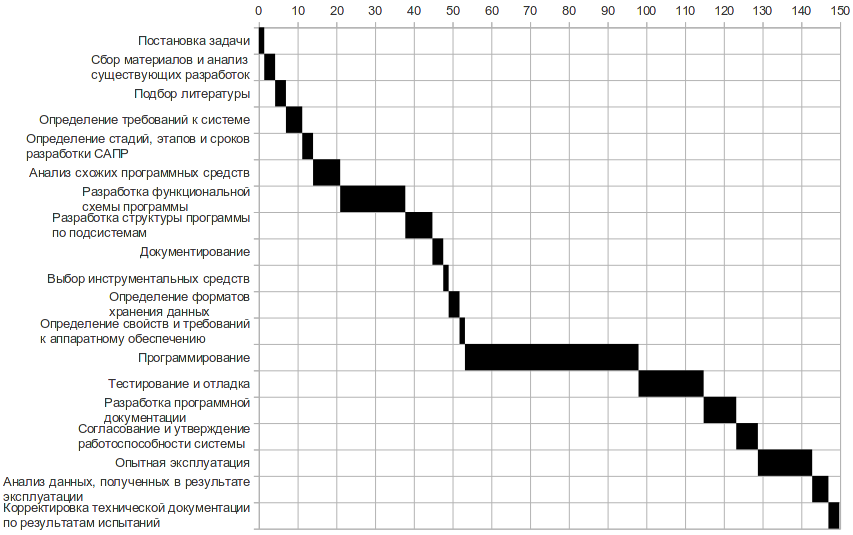
\includegraphics[width=0.98\textwidth]{diagrams/gantt.png}
  \caption{Диаграмма Ганта работы над проектом}
\end{figure}

\subsection{Расчет затрат на разработку} \label{sec:money-1}
\subsubsection{Расчет затрат на разработку программной системы}

Сметная стоимость проектирования и внедрения программы включает в себя следующие затраты, определяемые по формуле:
\begin{equation}
  C = C_{main} + C_{add} + C_{soc} + C_{mat} + C_{mach} + C_{n},
\end{equation}
\begin{ESKDexplanation}
  \item[где ] $C$~--- стоимость разработки ПО, руб.;
  \item $C_{main}$~--- основная заработная плата исполнителей, руб.;
  \item $C_{add}$~--- дополнительная заработная плата исполнителей, учитывающая потери времени на отпуска, руб.;
  \item $C_{soc}$~--- отчисления на социальные нужды, руб.;
  \item $C_{mat}$~--- затраты на используемые материалы, руб.;
  \item $C_{mach}$~--- затраты на  машинное время, руб.;
  \item $C_{n}$~--- накладные расходы включают затраты на управление, уборку, ремонт, электроэнергию, отопление и др., руб.
\end{ESKDexplanation}

Основная заработная плата исполнителей определяется по формуле:
\begin{equation}
  C_{main} = C_{a} \cdot T,
\end{equation}
\begin{ESKDexplanation}
  \item[где ] $С_{main}$~--- заработная плата исполнителей (руб.);
  \item $C_{a}$~--- средняя дневная оплата труда работника организации-разработчика программного продукта (1000 руб./чел.дн.);
  \item $T$ ~--- трудоемкость разработки программного продукта (чел.дн.).
\end{ESKDexplanation}

\begin{table}[H]
  \caption{Расчет основной заработной платы}
  \begin{tabular}{|p{0.18\textwidth}|p{0.15\textwidth}|p{0.15\textwidth}|p{0.2\textwidth}|p{0.2\textwidth}|}
  \hline
    Исполнитель & Оклад,\newline руб/мес. & Оклад, руб./дн. & Трудоемкость, чел.-дн. & Сумма, руб.
  \\ \hline
    Программист & 21000                   & 1000            & 107                    & 107000
  \\ \hline
    \multicolumn{4}{|c|}{Основная заработная плата исполнителя $C_{main}$}           & 107000
  \\ \hline
  \end{tabular}
\end{table}

Дополнительная заработная плата исполнителей, учитывающая потери времени на отпуска и болезни (принимается в среднем 15\% от основной заработной платы):

$C_{add} = 0,15 \cdot 107000 = 16050 (\fc{руб.})$

Отчисления на социальные нужды состоят из единого социального налога (ЕСН) и обязательного страхования от несчастных случаев и профессиональных заболеваний. ЕСН включает в себя отчисления во все внебюджетные фонды, в том числе пенсионный, обязательного медицинского страхования, социального страхования. Ставки налогов и их распределение определяются статьей 241 НК РФ.

Ставка налога рассчитывается, исходя из зарплаты сотрудника, при этом действует регрессивная шкала: чем больше зарплата, тем меньше налог.

Обычный размер ставки~--- для наемного работника, имеющего годовой доход менее 624 тыс. руб.~--- составляет 30\%. Типичный пример распределения этих денег для такого работника выглядит так:
\begin{itemize}
  \item Пенсионный фонд Российской Федерации~--- 22\%;
  \item Фонд социального страхования Российской Федерации~--- 2,9\%;
  \item Федеральный фонд обязательного медицинского страхования~--- 5,1\%.
\end{itemize}

Обязательное страхование от несчастных случаев на производстве и профессиональных заболеваний составляет 0,2\%.
Отчисления на социальные нужды рассчитываются относительно выплаченной заработной платы (суммы основной и дополнительной заработной платы) и составляют 30,2\%:

$C_{soc} = 0,302 \cdot (107000 + 16050) = 37161 (\fc{руб.})$

К затратам на используемые материалы относят затраты на магнитные носители данных, бумагу, канцтовары и др.
Затраты по ним определяются по экспертным оценкам.

\begin{table}[H]
  \caption{Расчет стоимости материалов}
  \begin{tabular}{|p{0.535\textwidth}|l|l|}
  \hline
    Материалы             & Количество, шт. & Стоимость, руб.
  \\ \hline
    Бумага писчая, пачек  & 2               & 400
  \\ \hline
    CD-диск               & 10              & 100
  \\ \hline
    Другие канцтовары     &~---             & 500
  \\ \hline
    \multicolumn{2}{|c|}{Общая стоимость материалов $C_{mat}$} & 1000
  \\ \hline
  \end{tabular}
\end{table}

Затраты на машинное время, необходимое для разработки ПО определяют как расходы на приобретение и подготовку материалов научно-технической информации.

Расчет затрат на машинное время осуществляется по формуле:
\begin{equation}
  C_{mach} = P_{mach} \cdot T ,
\end{equation}
\begin{ESKDexplanation}
  \item[где ] $P_{mach}$~--- себестоимость одного часа машинного времени, включающая в себя амортизацию технических средств, затраты на техническое обслуживание и стоимость электроэнергии;
  \item $T$~--- машинное время, используемое для проведение работ.
\end{ESKDexplanation}

Стоимость машинного дня принимается равным исходя из стоимости используемой ЭВМ.
Ноутбук ASUS X550VC принимается равным  22000 руб.
Норма амортизации 3 года, затраты на ремонт отсутствуют~--- в течении всего срока эксплуатации действует гарантия производителя.

Потребление подобного комплекта оборудования принимается равным 80 Вт/час.
При  стоимости 1 кВт$\cdot$ч согласно тарифам на электроэнергию в Ульяновске и Ульяновской области на 2014 год 2,85 руб., получаем

$P_{mach} = 6,84 (\fc{руб/час.})$

Необходимое количество машинного времени для реализации проекта по разработке программы рассчитывается по формуле:
\begin{equation}
  T = T_i \cdot t_{wd} \cdot T_a ,
\end{equation}
\begin{ESKDexplanation}
  \item[где ] $T_i$~--- трудоемкость работ, чел-дн;
  \item $t_{wd}$~--- продолжительность рабочей смены (при пятидневной рабочей неделе $t_{wd}$ = 8 ч);
  \item $T_a$ -- средний коэффициент использования машинного времени (принимается равным 1).
\end{ESKDexplanation}

Тогда

$T = 107 \cdot 8 \cdot 1 = 856 (\fc{ч.})$

Стоимость машинного времени составит:

$C_{mach} = 6,84 \cdot 856 = 5855 (\fc{руб.})$

К статье <<Накладные расходы>> относят расходы, связанные с управлением и организацией работ. Накладные расходы рассчитываются относительно основной заработной платы.
Величина накладных расходов принимается равной 85\% от основной зарплаты исполнителей.

Формула расчета:
\begin{equation}
  C_n = C_{main} \cdot K ,
\end{equation}
\begin{ESKDexplanation}
  \item[где ] $C_n$~--- накладные расходы, руб.;
  \item $C_{main}$~--- основная заработная плата исполнителей, руб.;
  \item $K$~--- коэффициент учета накладных расходов ($K = 0,85$).
\end{ESKDexplanation}

$C_n = 107000 \cdot 0,85 = 90950 (\fc{руб.})$

Результаты расчета затрат на проектирование программного обеспечения сведены в таблице \ref{table:cost-summary}.

\begin{table}[H]
  \caption{Смета затрат на разработку и внедрение программы}
  \label{table:cost-summary}
  \begin{tabular}{|p{0.623\textwidth}|l|l|}
  \hline
    Наименование статей             & Обозначение  & Сумма, руб.
  \\ \hline
    Основная заработная плата       & $C_{main}$   & 107000 \\ \hline
    Дополнительная заработная плата & $C_{add}$    & 16050  \\ \hline
    Отчисления на социальные нужды  & $C_{soc}$    & 37161  \\ \hline
    Материалы                       & $C_{mat}$    & 1000   \\ \hline
    Машинное время                  & $C_{mach}$   & 5855   \\ \hline
    Накладные расходы               & $C_n$        & 90950  \\ \hline
    \textbf{Итого}                  & $C$          & 258016 \\ \hline
  \end{tabular}
\end{table}

Таким образом, себестоимость разработки составляет 258016 руб.

Так как программа разрабатывается для внутреннего пользования и не будет продаваться в другие организации, то необходимость высчитывать ее оптовую и розничную цену отсутствует.

\subsection{Расчет основных технико-экономических показателей и эффективности использования программного продукта} \label{sec:money-2}

Экономический эффект~--- абсолютная величина, характеризующую достигнутые благодаря созданию или совершенствованию ПО дополнительные экономические результаты.

Экономическая эффективность~--- результативность экономической деятельности, экономических программ и мероприятий, характеризуемая отношением полученного экономического эффекта (результата) к затратам факторов (ресурсов), обусловившим получение этого результата.

Определим механизм возникновения экономического эффекта.
На кафедре <<Измерительно-вычислительные комплексы>> в учебном процессе задействованы компьютеры определенной конфигурации.

\begin{table}[H]
  \caption{Конфигурация ЭВМ}\label{table:pc-specs}
  \begin{tabular}{|l|p{0.72\textwidth}|}
    \hline
      \textbf{Компонент} & \textbf{Модель}
    \\ \hline
      Материнская плата  & Asus P5KPL-AM IN/ROEM/SI
    \\ \hline
      Процессор          & Intel(R) Core(TM)2 Duo CPU E7500 @ 2.93GHz (2 CPU)
    \\ \hline
      Модуль памяти      & DDR2 2038 MB RAM
    \\ \hline
      Жесткий диск       & Samsung HDD (320 GB, 7200 RPM, SATA-II)
    \\ \hline
      CD, DVD            &~---
    \\ \hline
      Монитор            & Philips Brilliance 19S
    \\ \hline
      Клавиатура         & Defender Magellan 920S PS/2
    \\ \hline
      Мышь               & Defender Flagman 110B PS/2
    \\ \hline
  \end{tabular}
\end{table}

Система автоматиизированного проектирования <<Altera Quartus II>>, используемая для работы с ПЛИС, обладает определенными системными требованиями.
Произведем соотношение этих показателей.

\begin{table}[H]
  \caption{Системные требования САПР <<Altera Quartus II>>}\label{table:compare-req}
  \begin{tabular}{|p{0.44\textwidth}|l|l|}
  \hline
    \textbf{Показатель}             & \textbf{Текущее значение} & \textbf{Требуемое значение}
  \\ \hline
    Тактовая частота процессора     & 2,9 GHz                   & 3,0 GHz
  \\ \hline
    Количество ядер процессора      & 2                         & 2
  \\ \hline
    Объем оперативной памяти        & 2 Gb                      & 4 Gb
  \\ \hline
  \end{tabular}
\end{table}

Как видно из таблицы \ref{table:compare-req}, для соответствия системным требованиям и обеспечения должной работоспособности улучшению (замене) должны подвергнуться процессор и ОЗУ ЭВМ.
Определим цену подобного улучшения.

Увеличения объема ОЗУ можно достичь путем покупки дополнительных модулей памяти~--- нет необходимости в полной замене существующих устройств.
Используем для улучшения модуль ОЗУ HYUNDAI / HYNIX DDR-II DIMM 2Gb <PC2-6400>.
Среднерыночная цена такого модуля памяти составляет 1010 руб.

Улучшение производительности ЦПУ без его замены невозможна: рассмотрим в качестве замены устройство CPU Intel Core 2 Duo E8400 3.0 GHz.
Среднерыночная цена данного процессора~--- 3863 руб.

Улучшению необходимо подвергнуть 24 ЭВМ.

\begin{equation}
  C_{hardware} = N \cdot (C_{RAM} + C_{CPU} + С_{inst}),
\end{equation}
\begin{ESKDexplanation}
  \item[где ] $C_{hardware}$~--- стоимость улучшения аппаратной части;
  \item $N$~--- количество ЭВМ для улучшения;
  \item $C_{RAM}$~--- среднерыночная цена одного выбранного модуля ОЗУ;
  \item $C_{CPU}$~--- среднерыночная цена одного выбранного ЦПУ;
  \item $C_{inst}$~--- стоимость проведения монтажных работ по установке нового оборудования.
\end{ESKDexplanation}

Работы по замене компонентов будут проводиться в сервисном центре.
Стоимость подобной работы, в виду ее сравнительной простоты, невелика и составляет в среднем 300 рублей.

Таким образом, стоимость улучшения аппаратной части равна:

$C_{hardware} = 24 \cdot (1010 + 3863 + 300) = 124152 (\fc{руб.})$

Будем исходить из предположения, что подобные улучшения не ведут к увеличению затрат на техническое обслуживание.

Несмотря на наличие бесплатных пробных версий <<Altera Quartus II>>, они не могут быть использованы в учебном процессе, так как предназначены исключительно для личного использования и должны быть удалены после истечения испытательного срока.

Стоимость коммерческой лицензии~--- 2995\$ (106670 руб.), она предоставляется на срок в 1 год, после чего должна быть продлена.
Стоимость продления лицензии~--- 2495\$ (88862 руб.), длительность данного продления~--- так же один год.

Таким образом, затраты на покупку САПР определяются следующим образом:

\begin{equation}
  C_{software} = C_{licence} + (N - 1) \cdot C_{renew},
\end{equation}
\begin{ESKDexplanation}
  \item[где ] $C_{software}$~--- стоимость покупки и обновления САПР;
  \item $C_{licence}$~--- стоимость покупки САПР;
  \item $N$~--- количество лет эксплуатации САПР;
  \item $C_{renew}$~--- стоимость обновления лицензии.
\end{ESKDexplanation}

Суммарные затраты на аппаратные улучшения и покупку САПР:

\begin{equation}
  C = C_{hardware} + C_{software},
\end{equation}
\begin{ESKDexplanation}
  \item[где ] $C$~--- суммарные затраты;
  \item $C_{hardware}$~--- стоимость аппаратных улучшений;
  \item $C_{software}$~--- стоимость покупки и обновления САПР.
\end{ESKDexplanation}

$C = 124512 + 106670 = 230822 (\fc{руб.})$

Разработка собственной системы, как видно из таблицы \ref{table:cost-summary}, обходится в 258016 рублей~--- таким образом, система покажет свою экономическую выгодность уже после первого года внедрения.
Ее использование позволит отказаться от аппаратного улучшения имеющихся ЭВМ и покупки дорогостоящих специализированных САПР.

Таким образом, можно сделать вывод, что разработка собственной системы экономически целесообразна, оправдана и выгодна.
Использование разрабатываемой программы позволяет намного облегчить работу студентов, сократить нагрузку на преподавателей и ведет к значительному сокращению денежных затрат по указанным ранее пунктам.